%% HELP WE'RE GOING TO DIE

\documentclass{article}
\usepackage{graphicx}
\usepackage{amsmath}

\usepackage{enumerate}
\usepackage{fullpage}

\title{CS181 Homework 2}
\author{Lucas Freitas and Angela Li}
\date{\today}

\begin{document}
\maketitle

\section{Perceptrons}

\begin{enumerate}

\item %% 1.1
The bright-or-dark feature \textbf{cannot} be recognized by a perceptron. Even using weights, the two features will be in a distribution that is not linearly separable. If we make weights be $1$, and input for a pixel be $1$ if the pixel is on, or $-1$ if it is off. The distribution would be similar to image below (credit to Lecture slides), considering blue dots to be data that is at least $75\%$ bright or dark, and red to be data that is not. 

\begin{figure}[h!]
\centering
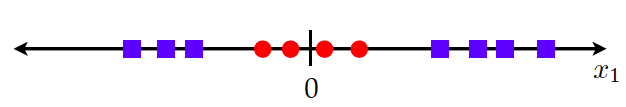
\includegraphics[width=80mm]{hw211.png}
\caption{Distribution of points for item $1$}
\end{figure}

It is easy to see that the data is not linearly separable, and the classification cannot be done with perceptrons alone. If we use high-level features, however, such that $\phi(x_i)=x_i^2$, the features become linearly separable (again, credit to Lecture slides):

\begin{figure}[h!]
\centering
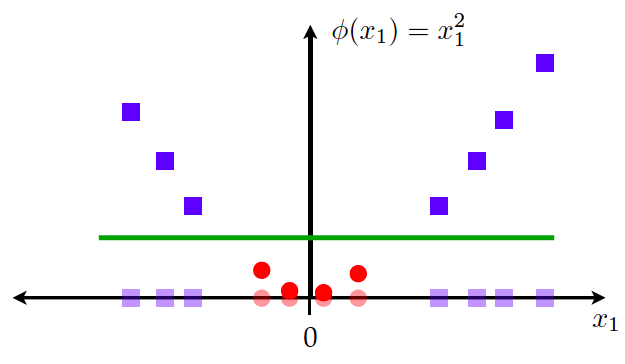
\includegraphics[width=80mm]{hw2112.png}
\caption{Distribution of points from item $1$ after applying $\phi(x_i)=x_i^2$}
\end{figure}

\item %% 1.2
The top-bright feature \textbf{can} be recognized by a perceptron. For this classification, we can use the following matrix of weights, considering that $x_i$ for each pixel is $1$ if the pixel is on, or $0$ if the pixel is off:

$$M=\begin{bmatrix}
      2&2&2           \\[0.3em]
      -1&-1&-1 \\[0.3em]
       -1&-1&-1
     \end{bmatrix}$$

That way, if $\sum_k{x_kw_k}$ is positive, we have a larger fraction of pixels on in the top row; otherwise, we know that there is not a larger fraction of pixels on in the top row.
x
\item %% 1.3
Just like in item $1$, connectedness \textbf{cannot} be recognized by a perceptron. Perceptrons are capable of viewing the local features of each pixel (checking whether it is on or off), but not at the relationships between two or more of them. That relationship is essential, however, for this classification problem, since connectedness depends on the combined configuration of adjacent pixels, which makes connectedness a non-linearly separable feature.

\end{enumerate}

\section{Learning Algorithms}
 
%% 2
\begin{itemize}

\item \textbf{Decision trees} \\ 
Decision trees are a viable candidate for the digit classification task.
%% argument

\item \textbf{Boosted decision stumps} \\
Boosted decision stumps are not a good candidate for the digit classification task.
%% argument

\item \textbf{Perceptrons} \\
Perceptrons are a viable candidate for the digit classification task.
%% argument

\item \textbf{Multi-layer feed-forward neural networks} \\
Multi-layer feed-forward neural networks are a great candidate for the digit classification task.
%% argument

\end{itemize}

\section{Neural Networks}

\begin{enumerate}

\item %% 3.1
See \texttt{FeedForward()}.

\item %% 3.2
See \texttt{Backprop()}.

\item %% 3.3
See \texttt{Train()}.

\item %% 3.4
See \texttt{EncodedNetworkFramework()}.

\item %% 3.5
In normalizing the input values from [0, 255] to between 0 and 1, we adapt them to the outputs of the sigmoid function, which is useful in calculating intermediary values. Normalization is also good because it preserves all relationships between inputs without introducing bias.
\newpage
\item %% 3.6
After trying learning rates of 1.0, 0.1, 0.01, and 0.001, we found that the learning rate exhibiting best performance was 0.1:

\begin{center}
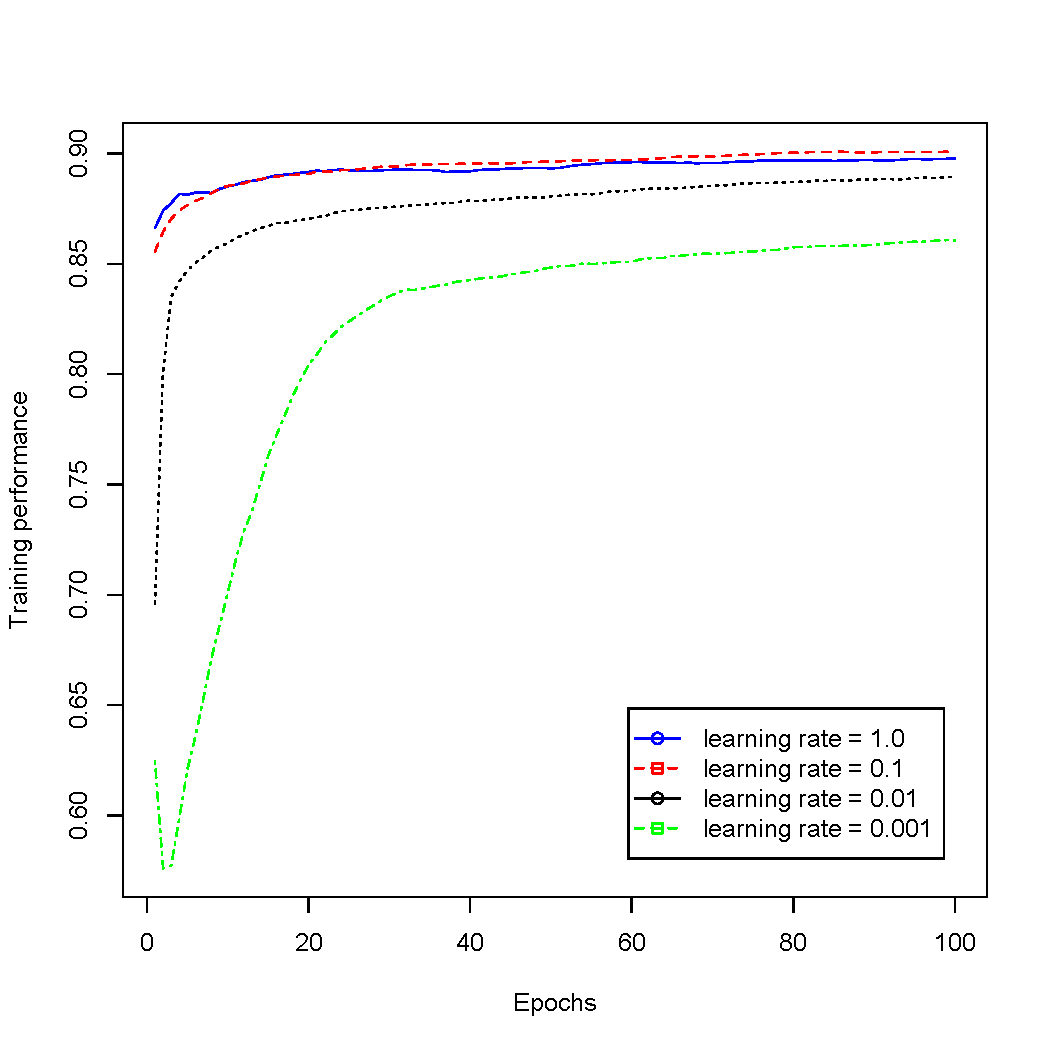
\includegraphics[width=75mm]{fig3.pdf} 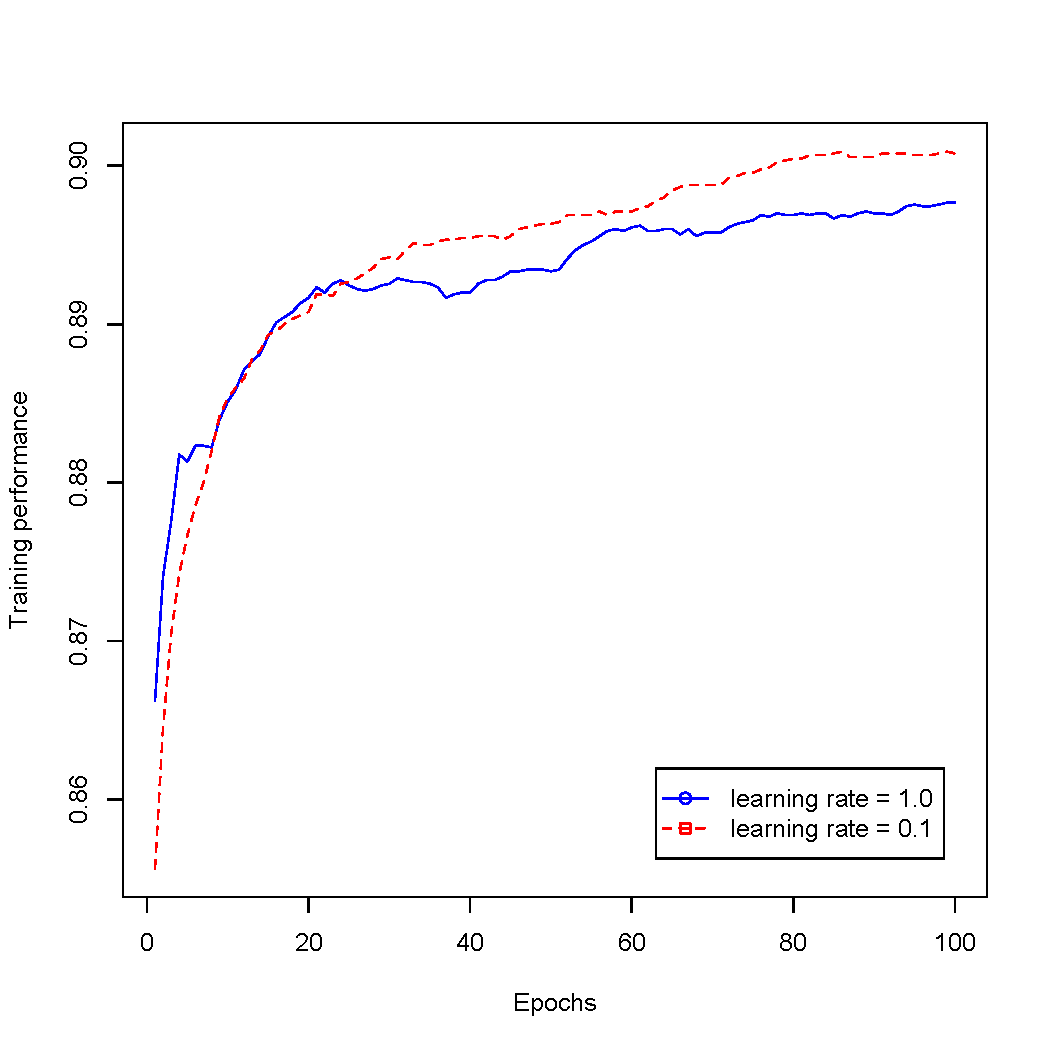
\includegraphics[width=75mm]{fig4.pdf}
\end{center}

\begin{enumerate}[(a)]

\item %% 3.6.a
The learning rate used is $0.1$.
 
\item %% 3.6.b
The graph of the training set and validation set $error$ against the number of epochs can be seen below:
\begin{center}
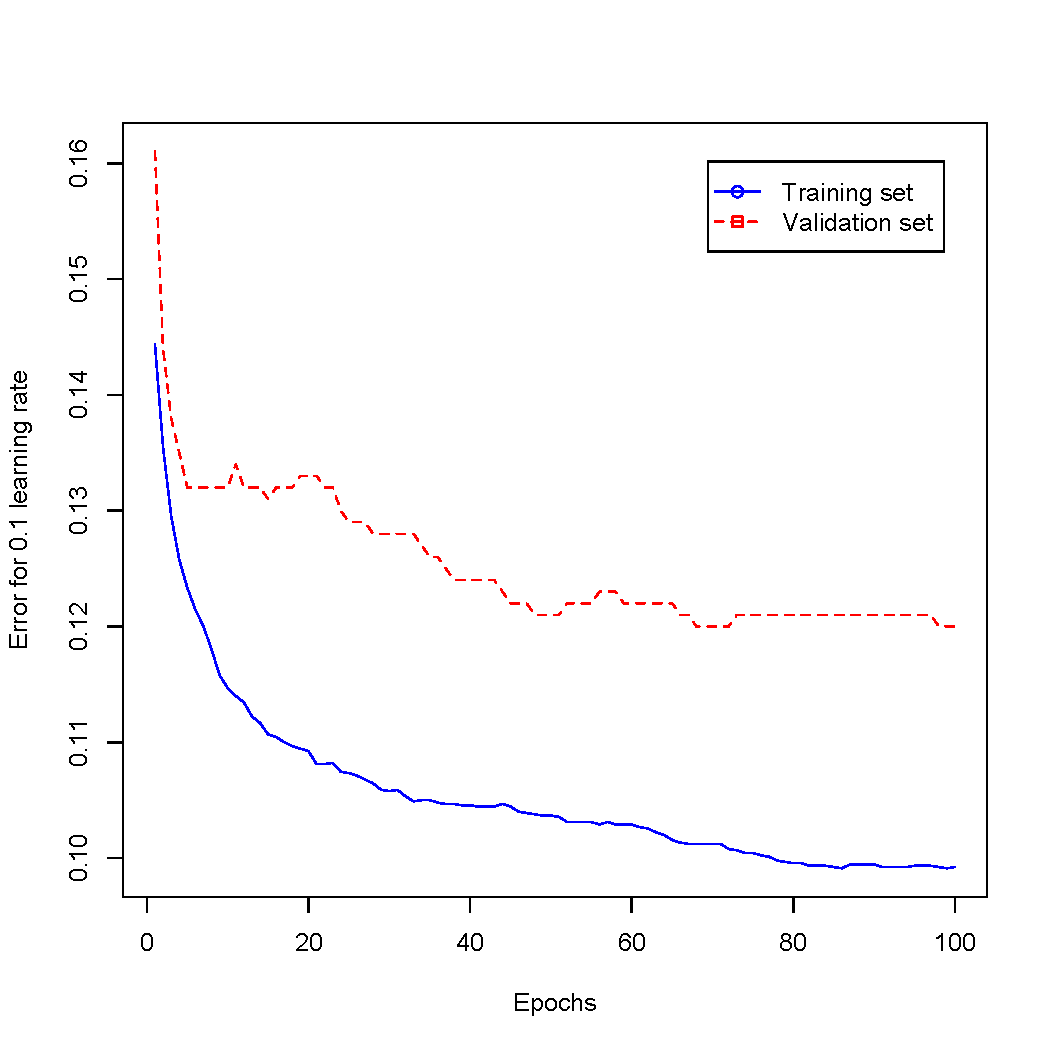
\includegraphics[width=75mm]{fig5.pdf}
\end{center}

\begin{enumerate}[i.]

\item %% 3.6.b.i
It does not appear that we are in danger of overfitting by training for too many epochs, as performance continues to increase (up to an apparent asymptotic upper bound) as the number of epochs we train for increases.

\item %% 3.6.b.ii
We thought that $50$ is a good number of epochs to train for since for larger number of epochs, the decrease in the error is not very significant, and running more epochs will just take a lot more time in the program execution, not actually improving its performance too much. 

\item %% 3.6.b.iii

\end{enumerate}

\item %% 3.6.c
For learning rate 0.1 and 50 epochs, our network had a training, validation, and test performance of 0.8964, 0.879, and 0.9160, respectively.

\end{enumerate}

\item

\begin{enumerate}[(a)]

\item %% 3.7.a
Running the algorithm for $15$ and $30$ hidden layers, and for a learning rate of $1.0, 0.1, 0.01,$ and $0.001$, we realized that the optimal learning rate would be $0.1$, just like in $6(a)$, for both $15$ or $30$ hidden layers.

\item %% 3.7.b
One way that we can go about doing that is by keeping track of the last $k$, let's say $10$, performances by epoch. Consider that we are looking at the $i_{th}$ performance, $P_i$. Let's also consider that $i>10$. We just need to check for each performance if:
$$\left| P_i-\frac{1}{10}\sum_{j=i-10}^{i-1}{P_j}\right|<t$$
Where $t$ is a threshold we pick. That is, we will perform the algorithm until $i==100$ or until we reach that threshold, which would mean that the increase in are seeing in the performance is now small, and we should stop iterating.

\item %% 3.7.c
Using a threshold $t=0.001$, we get $26$ epochs for $15$ hidden units, and $38$ epochs for $30$ hidden units. The graphs can be seen below:

\item %% 3.7.d

\item %% 3.7.e

\item %% 3.7.f

\end{enumerate}

\item

\begin{enumerate}[(a)]

\item %% 3.8.a

\item %% 3.8.b

\end{enumerate}

\end{enumerate}

\section{Error Functions}

\begin{enumerate}

\item %% 4.1

\item %% 4.2

\end{enumerate}

\end{document}